\subsection{Vermessung von Pedestals und Noise}
\label{sec:noise}

Als nächstes müssen Störsignale identifiziert werden. Dafür wird zunächst ein Überblick 
über die Pedestals und die Noise gegeben. Die Werte pro Streifen sind in 
Abbildung \ref{fig:pedestals} dargestellt. Zur Bestimmung, werden die aufgenommenen 
ADC Counts mit Hilfe von Gleichung \eqref{eqn:pedestal} in die Pedestals umgerechnet. 
Für die Noise bzw. für das Rauschen wird Formel \eqref{eqn:noise} verwendet.


\begin{figure}[H]
\centering
\begin{subfigure}{.5\textwidth}
  \centering
  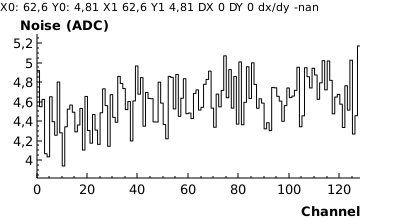
\includegraphics[width=\linewidth]{plots/noise.pdf}
\end{subfigure}%
\begin{subfigure}{.5\textwidth}
  \centering
  \includegraphics[width=\linewidth]{plots/pedestals.pdf}
\end{subfigure}
\caption{Pedestals und Noise für die einzelnen Steifen. Die Werte werden dabei jeweils mit 
Gleichung \eqref{eqn:pedestal} und Gleichung \eqref{eqn:noise} bestimmt.}
\label{fig:pedestals}
\end{figure}

Zur Berechnung des Rauschens, wird der Common Mode Shift benötigt. Dieser ist 
in Abbildung \ref{fig:shift} dargestellt und wird mittels Gleichung 
\eqref{eqn:shift} berechnet. Im allgemeinen wird angenommen, dass dieser 
Gaußverteilt um Null ist. Aus diesem Grund werden mit Hilfe von 
\texttt{numpy.random.normal} 99999999 gaußverteilte Zufallszahlen mit einem Mittelwert 
von 0 und der Varianz der Messwerte erstellt und als Vergleichsgauß über die Messwerte 
gelegt.

\begin{figure}[H]
  \centering
  \includegraphics[width=0.7\textwidth]{plots/cshift.pdf}
  \caption{Darstellung des Common Mode Shifts. Da theoretisch eine Gaußverteilung 
  um den Wert 0 erwartet wird, wird ein Theoriegauß zum Vergleich hinzugefügt, 
  der die Varianz der gemessenen Werte besitzt.}
  \label{fig:shift}
\end{figure}

Zu erkennen ist, dass die aufgenommenen Werte für den Common Mode Shift 
näherungsweise einer Gaußverteilung entsprechen.